\documentclass[1p]{elsarticle_modified}
%\bibliographystyle{elsarticle-num}

%\usepackage[colorlinks]{hyperref}
%\usepackage{abbrmath_seonhwa} %\Abb, \Ascr, \Acal ,\Abf, \Afrak
\usepackage{amsfonts}
\usepackage{amssymb}
\usepackage{amsmath}
\usepackage{amsthm}
\usepackage{scalefnt}
\usepackage{amsbsy}
\usepackage{kotex}
\usepackage{caption}
\usepackage{subfig}
\usepackage{color}
\usepackage{graphicx}
\usepackage{xcolor} %% white, black, red, green, blue, cyan, magenta, yellow
\usepackage{float}
\usepackage{setspace}
\usepackage{hyperref}

\usepackage{tikz}
\usetikzlibrary{arrows}

\usepackage{multirow}
\usepackage{array} % fixed length table
\usepackage{hhline}

%%%%%%%%%%%%%%%%%%%%%
\makeatletter
\renewcommand*\env@matrix[1][\arraystretch]{%
	\edef\arraystretch{#1}%
	\hskip -\arraycolsep
	\let\@ifnextchar\new@ifnextchar
	\array{*\c@MaxMatrixCols c}}
\makeatother %https://tex.stackexchange.com/questions/14071/how-can-i-increase-the-line-spacing-in-a-matrix
%%%%%%%%%%%%%%%

\usepackage[normalem]{ulem}

\newcommand{\msout}[1]{\ifmmode\text{\sout{\ensuremath{#1}}}\else\sout{#1}\fi}
%SOURCE: \msout is \stkout macro in https://tex.stackexchange.com/questions/20609/strikeout-in-math-mode

\newcommand{\cancel}[1]{
	\ifmmode
	{\color{red}\msout{#1}}
	\else
	{\color{red}\sout{#1}}
	\fi
}

\newcommand{\add}[1]{
	{\color{blue}\uwave{#1}}
}

\newcommand{\replace}[2]{
	\ifmmode
	{\color{red}\msout{#1}}{\color{blue}\uwave{#2}}
	\else
	{\color{red}\sout{#1}}{\color{blue}\uwave{#2}}
	\fi
}

\newcommand{\Sol}{\mathcal{S}} %segment
\newcommand{\D}{D} %diagram
\newcommand{\A}{\mathcal{A}} %arc


%%%%%%%%%%%%%%%%%%%%%%%%%%%%%5 test

\def\sl{\operatorname{\textup{SL}}(2,\Cbb)}
\def\psl{\operatorname{\textup{PSL}}(2,\Cbb)}
\def\quan{\mkern 1mu \triangleright \mkern 1mu}

\theoremstyle{definition}
\newtheorem{thm}{Theorem}[section]
\newtheorem{prop}[thm]{Proposition}
\newtheorem{lem}[thm]{Lemma}
\newtheorem{ques}[thm]{Question}
\newtheorem{cor}[thm]{Corollary}
\newtheorem{defn}[thm]{Definition}
\newtheorem{exam}[thm]{Example}
\newtheorem{rmk}[thm]{Remark}
\newtheorem{alg}[thm]{Algorithm}

\newcommand{\I}{\sqrt{-1}}
\begin{document}

%\begin{frontmatter}
%
%\title{Boundary parabolic representations of knots up to 8 crossings}
%
%%% Group authors per affiliation:
%\author{Yunhi Cho} 
%\address{Department of Mathematics, University of Seoul, Seoul, Korea}
%\ead{yhcho@uos.ac.kr}
%
%
%\author{Seonhwa Kim} %\fnref{s_kim}}
%\address{Center for Geometry and Physics, Institute for Basic Science, Pohang, 37673, Korea}
%\ead{ryeona17@ibs.re.kr}
%
%\author{Hyuk Kim}
%\address{Department of Mathematical Sciences, Seoul National University, Seoul 08826, Korea}
%\ead{hyukkim@snu.ac.kr}
%
%\author{Seokbeom Yoon}
%\address{Department of Mathematical Sciences, Seoul National University, Seoul, 08826,  Korea}
%\ead{sbyoon15@snu.ac.kr}
%
%\begin{abstract}
%We find all boundary parabolic representation of knots up to 8 crossings.
%
%\end{abstract}
%\begin{keyword}
%    \MSC[2010] 57M25 
%\end{keyword}
%
%\end{frontmatter}

%\linenumbers
%\tableofcontents
%
\newcommand\colored[1]{\textcolor{white}{\rule[-0.35ex]{0.8em}{1.4ex}}\kern-0.8em\color{red} #1}%
%\newcommand\colored[1]{\textcolor{white}{ #1}\kern-2.17ex	\textcolor{white}{ #1}\kern-1.81ex	\textcolor{white}{ #1}\kern-2.15ex\color{red}#1	}

{\Large $\underline{12a_{1172}~(K12a_{1172})}$}

\setlength{\tabcolsep}{10pt}
\renewcommand{\arraystretch}{1.6}
\vspace{1cm}\begin{tabular}{m{100pt}>{\centering\arraybackslash}m{274pt}}
\multirow{5}{120pt}{
	\centering
	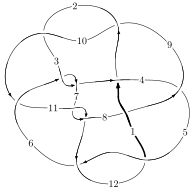
\includegraphics[width=112pt]{../../../GIT/diagram.site/Diagrams/png/1973_12a_1172.png}\\
\ \ \ A knot diagram\footnotemark}&
\allowdisplaybreaks
\textbf{Linearized knot diagam} \\
\cline{2-2}
 &
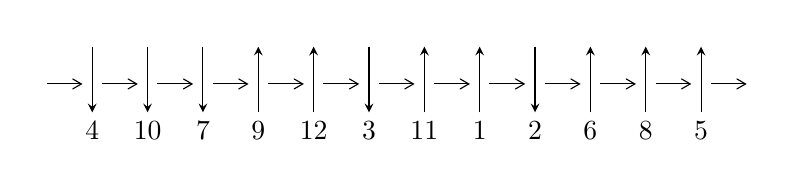
\begin{tikzpicture}[x=20pt, y=17pt]
	% nodes
	\node (C0) at (0, 0) {};
	\node (C1) at (1, 0) {};
	\node (C1U) at (1, +1) {};
	\node (C1D) at (1, -1) {4};

	\node (C2) at (2, 0) {};
	\node (C2U) at (2, +1) {};
	\node (C2D) at (2, -1) {10};

	\node (C3) at (3, 0) {};
	\node (C3U) at (3, +1) {};
	\node (C3D) at (3, -1) {7};

	\node (C4) at (4, 0) {};
	\node (C4U) at (4, +1) {};
	\node (C4D) at (4, -1) {9};

	\node (C5) at (5, 0) {};
	\node (C5U) at (5, +1) {};
	\node (C5D) at (5, -1) {12};

	\node (C6) at (6, 0) {};
	\node (C6U) at (6, +1) {};
	\node (C6D) at (6, -1) {3};

	\node (C7) at (7, 0) {};
	\node (C7U) at (7, +1) {};
	\node (C7D) at (7, -1) {11};

	\node (C8) at (8, 0) {};
	\node (C8U) at (8, +1) {};
	\node (C8D) at (8, -1) {1};

	\node (C9) at (9, 0) {};
	\node (C9U) at (9, +1) {};
	\node (C9D) at (9, -1) {2};

	\node (C10) at (10, 0) {};
	\node (C10U) at (10, +1) {};
	\node (C10D) at (10, -1) {6};

	\node (C11) at (11, 0) {};
	\node (C11U) at (11, +1) {};
	\node (C11D) at (11, -1) {8};

	\node (C12) at (12, 0) {};
	\node (C12U) at (12, +1) {};
	\node (C12D) at (12, -1) {5};
	\node (C13) at (13, 0) {};

	% arrows
	\draw[->,>={angle 60}]
	(C0) edge (C1) (C1) edge (C2) (C2) edge (C3) (C3) edge (C4) (C4) edge (C5) (C5) edge (C6) (C6) edge (C7) (C7) edge (C8) (C8) edge (C9) (C9) edge (C10) (C10) edge (C11) (C11) edge (C12) (C12) edge (C13) ;	\draw[->,>=stealth]
	(C1U) edge (C1D) (C2U) edge (C2D) (C3U) edge (C3D) (C4D) edge (C4U) (C5D) edge (C5U) (C6U) edge (C6D) (C7D) edge (C7U) (C8D) edge (C8U) (C9U) edge (C9D) (C10D) edge (C10U) (C11D) edge (C11U) (C12D) edge (C12U) ;
	\end{tikzpicture} \\
\hhline{~~} \\& 
\textbf{Solving Sequence} \\ \cline{2-2} 
 &
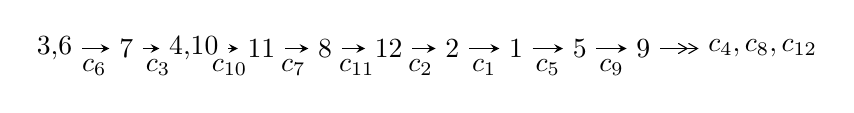
\begin{tikzpicture}[x=23pt, y=7pt]
	% node
	\node (A0) at (-1/8, 0) {3,6};
	\node (A1) at (1, 0) {7};
	\node (A2) at (33/16, 0) {4,10};
	\node (A3) at (25/8, 0) {11};
	\node (A4) at (33/8, 0) {8};
	\node (A5) at (41/8, 0) {12};
	\node (A6) at (49/8, 0) {2};
	\node (A7) at (57/8, 0) {1};
	\node (A8) at (65/8, 0) {5};
	\node (A9) at (73/8, 0) {9};
	\node (C1) at (1/2, -1) {$c_{6}$};
	\node (C2) at (3/2, -1) {$c_{3}$};
	\node (C3) at (21/8, -1) {$c_{10}$};
	\node (C4) at (29/8, -1) {$c_{7}$};
	\node (C5) at (37/8, -1) {$c_{11}$};
	\node (C6) at (45/8, -1) {$c_{2}$};
	\node (C7) at (53/8, -1) {$c_{1}$};
	\node (C8) at (61/8, -1) {$c_{5}$};
	\node (C9) at (69/8, -1) {$c_{9}$};
	\node (A10) at (11, 0) {$c_{4},c_{8},c_{12}$};

	% edge
	\draw[->,>=stealth]	
	(A0) edge (A1) (A1) edge (A2) (A2) edge (A3) (A3) edge (A4) (A4) edge (A5) (A5) edge (A6) (A6) edge (A7) (A7) edge (A8) (A8) edge (A9) ;
	\draw[->>,>={angle 60}]	
	(A9) edge (A10);
\end{tikzpicture} \\ 

\end{tabular} \\

\footnotetext{
The image of knot diagram is generated by the software ``\textbf{Draw programme}" developed by Andrew Bartholomew(\url{http://www.layer8.co.uk/maths/draw/index.htm\#Running-draw}), where we modified some parts for our purpose(\url{https://github.com/CATsTAILs/LinksPainter}).
}\phantom \\ \newline 
\centering \textbf{Ideals for irreducible components\footnotemark of $X_{\text{par}}$} 
 
\begin{align*}
I^u_{1}&=\langle 
1.26512\times10^{751} u^{149}+4.92723\times10^{751} u^{148}+\cdots+9.75259\times10^{750} b+3.75083\times10^{754},\\
\phantom{I^u_{1}}&\phantom{= \langle  }1.46795\times10^{755} u^{149}+6.05059\times10^{755} u^{148}+\cdots+3.54702\times10^{754} a+5.97136\times10^{758},\\
\phantom{I^u_{1}}&\phantom{= \langle  }u^{150}+5 u^{149}+\cdots+25271 u+3637\rangle \\
I^u_{2}&=\langle 
-5.55350\times10^{23} u^{39}-2.43477\times10^{24} u^{38}+\cdots+4.09608\times10^{22} b+5.26413\times10^{23},\\
\phantom{I^u_{2}}&\phantom{= \langle  }-3.66815\times10^{23} u^{39}-1.42903\times10^{24} u^{38}+\cdots+4.09608\times10^{22} a+7.74087\times10^{23},\\
\phantom{I^u_{2}}&\phantom{= \langle  }u^{40}+4 u^{39}+\cdots-13 u^2+1\rangle \\
\\
\end{align*}
\raggedright * 2 irreducible components of $\dim_{\mathbb{C}}=0$, with total 190 representations.\\
\footnotetext{All coefficients of polynomials are rational numbers. But the coefficients are sometimes approximated in decimal forms when there is not enough margin.}
\newpage
\renewcommand{\arraystretch}{1}
\centering \section*{I. $I^u_{1}= \langle 1.27\times10^{751} u^{149}+4.93\times10^{751} u^{148}+\cdots+9.75\times10^{750} b+3.75\times10^{754},\;1.47\times10^{755} u^{149}+6.05\times10^{755} u^{148}+\cdots+3.55\times10^{754} a+5.97\times10^{758},\;u^{150}+5 u^{149}+\cdots+25271 u+3637 \rangle$}
\flushleft \textbf{(i) Arc colorings}\\
\begin{tabular}{m{7pt} m{180pt} m{7pt} m{180pt} }
\flushright $a_{3}=$&$\begin{pmatrix}0\\u\end{pmatrix}$ \\
\flushright $a_{6}=$&$\begin{pmatrix}1\\0\end{pmatrix}$ \\
\flushright $a_{7}=$&$\begin{pmatrix}1\\u^2\end{pmatrix}$ \\
\flushright $a_{4}=$&$\begin{pmatrix}- u\\- u^3+u\end{pmatrix}$ \\
\flushright $a_{10}=$&$\begin{pmatrix}-4.13854 u^{149}-17.0582 u^{148}+\cdots-98334.7 u-16834.9\\-1.29722 u^{149}-5.05223 u^{148}+\cdots-23607.2 u-3845.99\end{pmatrix}$ \\
\flushright $a_{11}=$&$\begin{pmatrix}-5.43576 u^{149}-22.1105 u^{148}+\cdots-121942. u-20680.9\\-1.29722 u^{149}-5.05223 u^{148}+\cdots-23607.2 u-3845.99\end{pmatrix}$ \\
\flushright $a_{8}=$&$\begin{pmatrix}7.01380 u^{149}+28.8224 u^{148}+\cdots+162058. u+27707.0\\6.35386 u^{149}+26.1672 u^{148}+\cdots+148191. u+25334.3\end{pmatrix}$ \\
\flushright $a_{12}=$&$\begin{pmatrix}3.94062 u^{149}+16.2785 u^{148}+\cdots+89284.0 u+15295.2\\0.141724 u^{149}+0.883339 u^{148}+\cdots+7321.73 u+1509.73\end{pmatrix}$ \\
\flushright $a_{2}=$&$\begin{pmatrix}-1.44983 u^{149}-5.74168 u^{148}+\cdots-31453.2 u-5285.38\\-4.65175 u^{149}-18.9905 u^{148}+\cdots-109459. u-18606.0\end{pmatrix}$ \\
\flushright $a_{1}=$&$\begin{pmatrix}-5.14999 u^{149}-20.9229 u^{148}+\cdots-120587. u-20507.9\\-3.80366 u^{149}-15.5738 u^{148}+\cdots-90757.1 u-15456.8\end{pmatrix}$ \\
\flushright $a_{5}=$&$\begin{pmatrix}3.43640 u^{149}+14.2416 u^{148}+\cdots+76206.2 u+13142.3\\2.56694 u^{149}+10.6431 u^{148}+\cdots+62911.6 u+10837.4\end{pmatrix}$ \\
\flushright $a_{9}=$&$\begin{pmatrix}1.70084 u^{149}+6.62008 u^{148}+\cdots+29394.3 u+4671.47\\1.88565 u^{149}+7.77565 u^{148}+\cdots+42675.4 u+7307.30\end{pmatrix}$\\&\end{tabular}
\flushleft \textbf{(ii) Obstruction class $= -1$}\\~\\
\flushleft \textbf{(iii) Cusp Shapes $= 11.7905 u^{149}+47.9073 u^{148}+\cdots+263835. u+44679.3$}\\~\\
\newpage\renewcommand{\arraystretch}{1}
\flushleft \textbf{(iv) u-Polynomials at the component}\newline \\
\begin{tabular}{m{50pt}|m{274pt}}
Crossings & \hspace{64pt}u-Polynomials at each crossing \\
\hline $$\begin{aligned}c_{1}\end{aligned}$$&$\begin{aligned}
&u^{150}-11 u^{149}+\cdots+27517 u-277
\end{aligned}$\\
\hline $$\begin{aligned}c_{2},c_{9}\end{aligned}$$&$\begin{aligned}
&u^{150}-62 u^{148}+\cdots-11776 u+448
\end{aligned}$\\
\hline $$\begin{aligned}c_{3},c_{6}\end{aligned}$$&$\begin{aligned}
&u^{150}+5 u^{149}+\cdots+25271 u+3637
\end{aligned}$\\
\hline $$\begin{aligned}c_{4}\end{aligned}$$&$\begin{aligned}
&u^{150}+3 u^{149}+\cdots+1401453 u+97263
\end{aligned}$\\
\hline $$\begin{aligned}c_{5},c_{12}\end{aligned}$$&$\begin{aligned}
&u^{150}-3 u^{149}+\cdots+3773 u+227
\end{aligned}$\\
\hline $$\begin{aligned}c_{7},c_{11}\end{aligned}$$&$\begin{aligned}
&u^{150}-47 u^{148}+\cdots+242552 u+55892
\end{aligned}$\\
\hline $$\begin{aligned}c_{8}\end{aligned}$$&$\begin{aligned}
&u^{150}+3 u^{149}+\cdots+117 u+27
\end{aligned}$\\
\hline $$\begin{aligned}c_{10}\end{aligned}$$&$\begin{aligned}
&u^{150}+u^{149}+\cdots+5517033568 u+726291007
\end{aligned}$\\
\hline
\end{tabular}\\~\\
\newpage\renewcommand{\arraystretch}{1}
\flushleft \textbf{(v) Riley Polynomials at the component}\newline \\
\begin{tabular}{m{50pt}|m{274pt}}
Crossings & \hspace{64pt}Riley Polynomials at each crossing \\
\hline $$\begin{aligned}c_{1}\end{aligned}$$&$\begin{aligned}
&y^{150}- y^{149}+\cdots-661651313 y+76729
\end{aligned}$\\
\hline $$\begin{aligned}c_{2},c_{9}\end{aligned}$$&$\begin{aligned}
&y^{150}-124 y^{149}+\cdots-58378240 y+200704
\end{aligned}$\\
\hline $$\begin{aligned}c_{3},c_{6}\end{aligned}$$&$\begin{aligned}
&y^{150}-93 y^{149}+\cdots+1259345009 y+13227769
\end{aligned}$\\
\hline $$\begin{aligned}c_{4}\end{aligned}$$&$\begin{aligned}
&y^{150}+49 y^{149}+\cdots-447479481843 y+9460091169
\end{aligned}$\\
\hline $$\begin{aligned}c_{5},c_{12}\end{aligned}$$&$\begin{aligned}
&y^{150}+109 y^{149}+\cdots+1029767 y+51529
\end{aligned}$\\
\hline $$\begin{aligned}c_{7},c_{11}\end{aligned}$$&$\begin{aligned}
&y^{150}-94 y^{149}+\cdots-105400910672 y+3123915664
\end{aligned}$\\
\hline $$\begin{aligned}c_{8}\end{aligned}$$&$\begin{aligned}
&y^{150}- y^{149}+\cdots+27513 y+729
\end{aligned}$\\
\hline $$\begin{aligned}c_{10}\end{aligned}$$&$\begin{aligned}
&y^{150}+49 y^{149}+\cdots+2.26\times10^{19} y+5.27\times10^{17}
\end{aligned}$\\
\hline
\end{tabular}\\~\\
\newpage\flushleft \textbf{(vi) Complex Volumes and Cusp Shapes}
$$\begin{array}{c|c|c}  
\text{Solutions to }I^u_{1}& \I (\text{vol} + \sqrt{-1}CS) & \text{Cusp shape}\\
 \hline 
\begin{aligned}
u &= \phantom{-}1.010160 + 0.001327 I \\
a &= -1.75230 - 0.22716 I \\
b &= \phantom{-}0.552597 - 0.775648 I\end{aligned}
 & -6.58473 - 0.02848 I & \phantom{-0.000000 } 0 \\ \hline\begin{aligned}
u &= \phantom{-}1.010160 - 0.001327 I \\
a &= -1.75230 + 0.22716 I \\
b &= \phantom{-}0.552597 + 0.775648 I\end{aligned}
 & -6.58473 + 0.02848 I & \phantom{-0.000000 } 0 \\ \hline\begin{aligned}
u &= -0.986489 + 0.066960 I \\
a &= -1.274150 + 0.028000 I \\
b &= \phantom{-}2.16405 - 0.90350 I\end{aligned}
 & \phantom{-}0.12677 + 2.90266 I & \phantom{-0.000000 } 0 \\ \hline\begin{aligned}
u &= -0.986489 - 0.066960 I \\
a &= -1.274150 - 0.028000 I \\
b &= \phantom{-}2.16405 + 0.90350 I\end{aligned}
 & \phantom{-}0.12677 - 2.90266 I & \phantom{-0.000000 } 0 \\ \hline\begin{aligned}
u &= -0.119280 + 0.963787 I \\
a &= \phantom{-}0.099277 + 1.380620 I \\
b &= -0.626734 - 0.783400 I\end{aligned}
 & -3.62768 + 4.13150 I & \phantom{-0.000000 } 0 \\ \hline\begin{aligned}
u &= -0.119280 - 0.963787 I \\
a &= \phantom{-}0.099277 - 1.380620 I \\
b &= -0.626734 + 0.783400 I\end{aligned}
 & -3.62768 - 4.13150 I & \phantom{-0.000000 } 0 \\ \hline\begin{aligned}
u &= -0.737777 + 0.719467 I \\
a &= \phantom{-}0.268764 + 0.035848 I \\
b &= -0.703268 + 0.646362 I\end{aligned}
 & \phantom{-}3.69554 + 2.21429 I & \phantom{-0.000000 } 0 \\ \hline\begin{aligned}
u &= -0.737777 - 0.719467 I \\
a &= \phantom{-}0.268764 - 0.035848 I \\
b &= -0.703268 - 0.646362 I\end{aligned}
 & \phantom{-}3.69554 - 2.21429 I & \phantom{-0.000000 } 0 \\ \hline\begin{aligned}
u &= \phantom{-}0.938985 + 0.427249 I \\
a &= -0.946853 - 0.614308 I \\
b &= \phantom{-}0.94381 - 1.59285 I\end{aligned}
 & -1.36518 + 1.23438 I & \phantom{-0.000000 } 0 \\ \hline\begin{aligned}
u &= \phantom{-}0.938985 - 0.427249 I \\
a &= -0.946853 + 0.614308 I \\
b &= \phantom{-}0.94381 + 1.59285 I\end{aligned}
 & -1.36518 - 1.23438 I & \phantom{-0.000000 } 0\\
 \hline 
 \end{array}$$\newpage$$\begin{array}{c|c|c}  
\text{Solutions to }I^u_{1}& \I (\text{vol} + \sqrt{-1}CS) & \text{Cusp shape}\\
 \hline 
\begin{aligned}
u &= \phantom{-}0.957385 + 0.105545 I \\
a &= -1.224200 - 0.152693 I \\
b &= \phantom{-}2.61460 - 0.05986 I\end{aligned}
 & -2.40883 - 8.55995 I & \phantom{-0.000000 } 0 \\ \hline\begin{aligned}
u &= \phantom{-}0.957385 - 0.105545 I \\
a &= -1.224200 + 0.152693 I \\
b &= \phantom{-}2.61460 + 0.05986 I\end{aligned}
 & -2.40883 + 8.55995 I & \phantom{-0.000000 } 0 \\ \hline\begin{aligned}
u &= \phantom{-}0.998838 + 0.292870 I \\
a &= -0.601572 - 0.901246 I \\
b &= \phantom{-}0.472808 - 0.556492 I\end{aligned}
 & -1.07866 - 3.62942 I & \phantom{-0.000000 } 0 \\ \hline\begin{aligned}
u &= \phantom{-}0.998838 - 0.292870 I \\
a &= -0.601572 + 0.901246 I \\
b &= \phantom{-}0.472808 + 0.556492 I\end{aligned}
 & -1.07866 + 3.62942 I & \phantom{-0.000000 } 0 \\ \hline\begin{aligned}
u &= \phantom{-}0.399736 + 0.866442 I \\
a &= -0.562313 - 0.384015 I \\
b &= \phantom{-}0.962382 + 0.449510 I\end{aligned}
 & \phantom{-}5.61645 + 2.73061 I & \phantom{-0.000000 } 0 \\ \hline\begin{aligned}
u &= \phantom{-}0.399736 - 0.866442 I \\
a &= -0.562313 + 0.384015 I \\
b &= \phantom{-}0.962382 - 0.449510 I\end{aligned}
 & \phantom{-}5.61645 - 2.73061 I & \phantom{-0.000000 } 0 \\ \hline\begin{aligned}
u &= -0.827895 + 0.470631 I \\
a &= -0.419188 - 0.213084 I \\
b &= -0.86315 + 1.61563 I\end{aligned}
 & \phantom{-}3.23023 + 1.99379 I & \phantom{-0.000000 } 0 \\ \hline\begin{aligned}
u &= -0.827895 - 0.470631 I \\
a &= -0.419188 + 0.213084 I \\
b &= -0.86315 - 1.61563 I\end{aligned}
 & \phantom{-}3.23023 - 1.99379 I & \phantom{-0.000000 } 0 \\ \hline\begin{aligned}
u &= -0.176065 + 0.932223 I \\
a &= -0.546997 - 1.119370 I \\
b &= \phantom{-}0.368260 + 0.700906 I\end{aligned}
 & -1.86777 + 4.08465 I & \phantom{-0.000000 } 0 \\ \hline\begin{aligned}
u &= -0.176065 - 0.932223 I \\
a &= -0.546997 + 1.119370 I \\
b &= \phantom{-}0.368260 - 0.700906 I\end{aligned}
 & -1.86777 - 4.08465 I & \phantom{-0.000000 } 0\\
 \hline 
 \end{array}$$\newpage$$\begin{array}{c|c|c}  
\text{Solutions to }I^u_{1}& \I (\text{vol} + \sqrt{-1}CS) & \text{Cusp shape}\\
 \hline 
\begin{aligned}
u &= -0.932265 + 0.169371 I \\
a &= \phantom{-}0.61464 + 1.75356 I \\
b &= \phantom{-}0.393835 + 0.238423 I\end{aligned}
 & -2.58412 + 4.82057 I & \phantom{-0.000000 } 0 \\ \hline\begin{aligned}
u &= -0.932265 - 0.169371 I \\
a &= \phantom{-}0.61464 - 1.75356 I \\
b &= \phantom{-}0.393835 - 0.238423 I\end{aligned}
 & -2.58412 - 4.82057 I & \phantom{-0.000000 } 0 \\ \hline\begin{aligned}
u &= -1.048040 + 0.169863 I \\
a &= -0.85088 + 1.38483 I \\
b &= \phantom{-}0.250228 + 0.748347 I\end{aligned}
 & -4.81324 + 5.56239 I & \phantom{-0.000000 } 0 \\ \hline\begin{aligned}
u &= -1.048040 - 0.169863 I \\
a &= -0.85088 - 1.38483 I \\
b &= \phantom{-}0.250228 - 0.748347 I\end{aligned}
 & -4.81324 - 5.56239 I & \phantom{-0.000000 } 0 \\ \hline\begin{aligned}
u &= -0.928918 + 0.085232 I \\
a &= -1.084560 - 0.650075 I \\
b &= -0.643149 - 1.167960 I\end{aligned}
 & \phantom{-}0.26194 - 2.19269 I & \phantom{-0.000000 } 0 \\ \hline\begin{aligned}
u &= -0.928918 - 0.085232 I \\
a &= -1.084560 + 0.650075 I \\
b &= -0.643149 + 1.167960 I\end{aligned}
 & \phantom{-}0.26194 + 2.19269 I & \phantom{-0.000000 } 0 \\ \hline\begin{aligned}
u &= -0.923812 + 0.115947 I \\
a &= \phantom{-}0.981095 + 0.202493 I \\
b &= -1.85969 + 0.55662 I\end{aligned}
 & -0.41992 + 2.90044 I & \phantom{-0.000000 } 0 \\ \hline\begin{aligned}
u &= -0.923812 - 0.115947 I \\
a &= \phantom{-}0.981095 - 0.202493 I \\
b &= -1.85969 - 0.55662 I\end{aligned}
 & -0.41992 - 2.90044 I & \phantom{-0.000000 } 0 \\ \hline\begin{aligned}
u &= \phantom{-}0.904769 + 0.195901 I \\
a &= \phantom{-}0.806718 - 1.097620 I \\
b &= \phantom{-}0.046242 - 0.544135 I\end{aligned}
 & \phantom{-}1.64079 - 1.76353 I & \phantom{-0.000000 } 0 \\ \hline\begin{aligned}
u &= \phantom{-}0.904769 - 0.195901 I \\
a &= \phantom{-}0.806718 + 1.097620 I \\
b &= \phantom{-}0.046242 + 0.544135 I\end{aligned}
 & \phantom{-}1.64079 + 1.76353 I & \phantom{-0.000000 } 0\\
 \hline 
 \end{array}$$\newpage$$\begin{array}{c|c|c}  
\text{Solutions to }I^u_{1}& \I (\text{vol} + \sqrt{-1}CS) & \text{Cusp shape}\\
 \hline 
\begin{aligned}
u &= -0.823699 + 0.694777 I \\
a &= \phantom{-}0.620668 + 0.478797 I \\
b &= \phantom{-}0.421267 - 1.238130 I\end{aligned}
 & -0.36032 + 2.64753 I & \phantom{-0.000000 } 0 \\ \hline\begin{aligned}
u &= -0.823699 - 0.694777 I \\
a &= \phantom{-}0.620668 - 0.478797 I \\
b &= \phantom{-}0.421267 + 1.238130 I\end{aligned}
 & -0.36032 - 2.64753 I & \phantom{-0.000000 } 0 \\ \hline\begin{aligned}
u &= -0.329008 + 1.028150 I \\
a &= -0.210408 - 0.188365 I \\
b &= \phantom{-}0.595601 + 0.084418 I\end{aligned}
 & \phantom{-}1.52233 + 4.09710 I & \phantom{-0.000000 } 0 \\ \hline\begin{aligned}
u &= -0.329008 - 1.028150 I \\
a &= -0.210408 + 0.188365 I \\
b &= \phantom{-}0.595601 - 0.084418 I\end{aligned}
 & \phantom{-}1.52233 - 4.09710 I & \phantom{-0.000000 } 0 \\ \hline\begin{aligned}
u &= \phantom{-}0.887346 + 0.227586 I \\
a &= -0.812711 + 0.964936 I \\
b &= -1.189660 + 0.551074 I\end{aligned}
 & -2.43795 + 7.14768 I & \phantom{-0.000000 } 0 \\ \hline\begin{aligned}
u &= \phantom{-}0.887346 - 0.227586 I \\
a &= -0.812711 - 0.964936 I \\
b &= -1.189660 - 0.551074 I\end{aligned}
 & -2.43795 - 7.14768 I & \phantom{-0.000000 } 0 \\ \hline\begin{aligned}
u &= \phantom{-}0.795254 + 0.737819 I \\
a &= \phantom{-}0.864722 - 0.612025 I \\
b &= \phantom{-}0.41745 + 1.72341 I\end{aligned}
 & \phantom{-}0.02417 - 2.76819 I & \phantom{-0.000000 } 0 \\ \hline\begin{aligned}
u &= \phantom{-}0.795254 - 0.737819 I \\
a &= \phantom{-}0.864722 + 0.612025 I \\
b &= \phantom{-}0.41745 - 1.72341 I\end{aligned}
 & \phantom{-}0.02417 + 2.76819 I & \phantom{-0.000000 } 0 \\ \hline\begin{aligned}
u &= -0.133091 + 0.895417 I \\
a &= -0.17218 + 1.51826 I \\
b &= \phantom{-}0.808299 - 1.004490 I\end{aligned}
 & -4.47954 - 4.44672 I & \phantom{-0.000000 } 0 \\ \hline\begin{aligned}
u &= -0.133091 - 0.895417 I \\
a &= -0.17218 - 1.51826 I \\
b &= \phantom{-}0.808299 + 1.004490 I\end{aligned}
 & -4.47954 + 4.44672 I & \phantom{-0.000000 } 0\\
 \hline 
 \end{array}$$\newpage$$\begin{array}{c|c|c}  
\text{Solutions to }I^u_{1}& \I (\text{vol} + \sqrt{-1}CS) & \text{Cusp shape}\\
 \hline 
\begin{aligned}
u &= \phantom{-}0.185248 + 1.081780 I \\
a &= -0.465084 + 1.124470 I \\
b &= \phantom{-}0.128815 - 1.149810 I\end{aligned}
 & -6.66260 - 7.20467 I & \phantom{-0.000000 } 0 \\ \hline\begin{aligned}
u &= \phantom{-}0.185248 - 1.081780 I \\
a &= -0.465084 - 1.124470 I \\
b &= \phantom{-}0.128815 + 1.149810 I\end{aligned}
 & -6.66260 + 7.20467 I & \phantom{-0.000000 } 0 \\ \hline\begin{aligned}
u &= -1.003260 + 0.474064 I \\
a &= -0.426046 + 0.538649 I \\
b &= \phantom{-}0.315500 + 1.219820 I\end{aligned}
 & \phantom{-}2.69954 + 2.37915 I & \phantom{-0.000000 } 0 \\ \hline\begin{aligned}
u &= -1.003260 - 0.474064 I \\
a &= -0.426046 - 0.538649 I \\
b &= \phantom{-}0.315500 - 1.219820 I\end{aligned}
 & \phantom{-}2.69954 - 2.37915 I & \phantom{-0.000000 } 0 \\ \hline\begin{aligned}
u &= \phantom{-}0.865794 + 0.192350 I \\
a &= \phantom{-}0.819425 - 0.606169 I \\
b &= -0.79091 - 1.26456 I\end{aligned}
 & \phantom{-}1.25757 - 0.97218 I & \phantom{-0.000000 } 0 \\ \hline\begin{aligned}
u &= \phantom{-}0.865794 - 0.192350 I \\
a &= \phantom{-}0.819425 + 0.606169 I \\
b &= -0.79091 + 1.26456 I\end{aligned}
 & \phantom{-}1.25757 + 0.97218 I & \phantom{-0.000000 } 0 \\ \hline\begin{aligned}
u &= -0.943677 + 0.599804 I \\
a &= \phantom{-}0.717080 - 0.005338 I \\
b &= -0.155684 - 1.184590 I\end{aligned}
 & -0.58977 + 2.66247 I & \phantom{-0.000000 } 0 \\ \hline\begin{aligned}
u &= -0.943677 - 0.599804 I \\
a &= \phantom{-}0.717080 + 0.005338 I \\
b &= -0.155684 + 1.184590 I\end{aligned}
 & -0.58977 - 2.66247 I & \phantom{-0.000000 } 0 \\ \hline\begin{aligned}
u &= -1.056960 + 0.373139 I \\
a &= -0.0767874 - 0.0112237 I \\
b &= \phantom{-}0.149753 - 0.395142 I\end{aligned}
 & -1.83357 + 1.32917 I & \phantom{-0.000000 } 0 \\ \hline\begin{aligned}
u &= -1.056960 - 0.373139 I \\
a &= -0.0767874 + 0.0112237 I \\
b &= \phantom{-}0.149753 + 0.395142 I\end{aligned}
 & -1.83357 - 1.32917 I & \phantom{-0.000000 } 0\\
 \hline 
 \end{array}$$\newpage$$\begin{array}{c|c|c}  
\text{Solutions to }I^u_{1}& \I (\text{vol} + \sqrt{-1}CS) & \text{Cusp shape}\\
 \hline 
\begin{aligned}
u &= \phantom{-}1.051200 + 0.431460 I \\
a &= -0.129576 - 0.816108 I \\
b &= \phantom{-}1.068610 - 0.146172 I\end{aligned}
 & -2.27203 - 3.43715 I & \phantom{-0.000000 } 0 \\ \hline\begin{aligned}
u &= \phantom{-}1.051200 - 0.431460 I \\
a &= -0.129576 + 0.816108 I \\
b &= \phantom{-}1.068610 + 0.146172 I\end{aligned}
 & -2.27203 + 3.43715 I & \phantom{-0.000000 } 0 \\ \hline\begin{aligned}
u &= \phantom{-}0.704303 + 0.492491 I \\
a &= -0.116439 + 1.065210 I \\
b &= -1.62386 - 0.96825 I\end{aligned}
 & -0.60602 - 5.09602 I & \phantom{-0.000000 } 0 \\ \hline\begin{aligned}
u &= \phantom{-}0.704303 - 0.492491 I \\
a &= -0.116439 - 1.065210 I \\
b &= -1.62386 + 0.96825 I\end{aligned}
 & -0.60602 + 5.09602 I & \phantom{-0.000000 } 0 \\ \hline\begin{aligned}
u &= -1.118110 + 0.308233 I \\
a &= -0.277390 + 0.932094 I \\
b &= \phantom{-}0.979330 + 0.702422 I\end{aligned}
 & -3.24364 + 3.44616 I & \phantom{-0.000000 } 0 \\ \hline\begin{aligned}
u &= -1.118110 - 0.308233 I \\
a &= -0.277390 - 0.932094 I \\
b &= \phantom{-}0.979330 - 0.702422 I\end{aligned}
 & -3.24364 - 3.44616 I & \phantom{-0.000000 } 0 \\ \hline\begin{aligned}
u &= -0.328008 + 0.753116 I \\
a &= -0.902327 + 0.597892 I \\
b &= \phantom{-}1.165830 - 0.618355 I\end{aligned}
 & \phantom{-}1.37688 - 8.62221 I & \phantom{-0.000000 } 0 \\ \hline\begin{aligned}
u &= -0.328008 - 0.753116 I \\
a &= -0.902327 - 0.597892 I \\
b &= \phantom{-}1.165830 + 0.618355 I\end{aligned}
 & \phantom{-}1.37688 + 8.62221 I & \phantom{-0.000000 } 0 \\ \hline\begin{aligned}
u &= -0.810080 + 0.133797 I \\
a &= \phantom{-}0.661039 + 0.801510 I \\
b &= \phantom{-}0.433775 + 1.096310 I\end{aligned}
 & -0.24584 - 1.40229 I & \phantom{-0.000000 } 0 \\ \hline\begin{aligned}
u &= -0.810080 - 0.133797 I \\
a &= \phantom{-}0.661039 - 0.801510 I \\
b &= \phantom{-}0.433775 - 1.096310 I\end{aligned}
 & -0.24584 + 1.40229 I & \phantom{-0.000000 } 0\\
 \hline 
 \end{array}$$\newpage$$\begin{array}{c|c|c}  
\text{Solutions to }I^u_{1}& \I (\text{vol} + \sqrt{-1}CS) & \text{Cusp shape}\\
 \hline 
\begin{aligned}
u &= \phantom{-}1.125690 + 0.405810 I \\
a &= -0.212320 - 0.909509 I \\
b &= \phantom{-}0.465953 - 0.871792 I\end{aligned}
 & \phantom{-}0.12094 - 6.12459 I & \phantom{-0.000000 } 0 \\ \hline\begin{aligned}
u &= \phantom{-}1.125690 - 0.405810 I \\
a &= -0.212320 + 0.909509 I \\
b &= \phantom{-}0.465953 + 0.871792 I\end{aligned}
 & \phantom{-}0.12094 + 6.12459 I & \phantom{-0.000000 } 0 \\ \hline\begin{aligned}
u &= \phantom{-}1.200320 + 0.101588 I \\
a &= -0.130187 + 0.289602 I \\
b &= \phantom{-}0.305142 + 1.269170 I\end{aligned}
 & -6.75098 + 1.92609 I & \phantom{-0.000000 } 0 \\ \hline\begin{aligned}
u &= \phantom{-}1.200320 - 0.101588 I \\
a &= -0.130187 - 0.289602 I \\
b &= \phantom{-}0.305142 - 1.269170 I\end{aligned}
 & -6.75098 - 1.92609 I & \phantom{-0.000000 } 0 \\ \hline\begin{aligned}
u &= -0.080882 + 0.790242 I \\
a &= \phantom{-}0.10018 - 1.75276 I \\
b &= -0.029925 + 1.159940 I\end{aligned}
 & -7.75192 + 0.06941 I & \phantom{-0.000000 } 0 \\ \hline\begin{aligned}
u &= -0.080882 - 0.790242 I \\
a &= \phantom{-}0.10018 + 1.75276 I \\
b &= -0.029925 - 1.159940 I\end{aligned}
 & -7.75192 - 0.06941 I & \phantom{-0.000000 } 0 \\ \hline\begin{aligned}
u &= \phantom{-}0.790903\phantom{ +0.000000I} \\
a &= \phantom{-}1.65888\phantom{ +0.000000I} \\
b &= -1.23443\phantom{ +0.000000I}\end{aligned}
 & \phantom{-}2.40030\phantom{ +0.000000I} & \phantom{-0.000000 } 0 \\ \hline\begin{aligned}
u &= -0.768103 + 0.145727 I \\
a &= \phantom{-}1.95529 - 0.92787 I \\
b &= -1.204540 - 0.151735 I\end{aligned}
 & -2.01380 - 3.01029 I & \phantom{-0.000000 } 0 \\ \hline\begin{aligned}
u &= -0.768103 - 0.145727 I \\
a &= \phantom{-}1.95529 + 0.92787 I \\
b &= -1.204540 + 0.151735 I\end{aligned}
 & -2.01380 + 3.01029 I & \phantom{-0.000000 } 0 \\ \hline\begin{aligned}
u &= -0.197554 + 1.205700 I \\
a &= \phantom{-}0.118695 - 1.167590 I \\
b &= -0.618277 + 1.032640 I\end{aligned}
 & -3.51177 - 13.09830 I & \phantom{-0.000000 } 0\\
 \hline 
 \end{array}$$\newpage$$\begin{array}{c|c|c}  
\text{Solutions to }I^u_{1}& \I (\text{vol} + \sqrt{-1}CS) & \text{Cusp shape}\\
 \hline 
\begin{aligned}
u &= -0.197554 - 1.205700 I \\
a &= \phantom{-}0.118695 + 1.167590 I \\
b &= -0.618277 - 1.032640 I\end{aligned}
 & -3.51177 + 13.09830 I & \phantom{-0.000000 } 0 \\ \hline\begin{aligned}
u &= -1.137090 + 0.483728 I \\
a &= \phantom{-}0.705841 - 0.822951 I \\
b &= -0.902469 - 1.043400 I\end{aligned}
 & -1.11967 + 13.28180 I & \phantom{-0.000000 } 0 \\ \hline\begin{aligned}
u &= -1.137090 - 0.483728 I \\
a &= \phantom{-}0.705841 + 0.822951 I \\
b &= -0.902469 + 1.043400 I\end{aligned}
 & -1.11967 - 13.28180 I & \phantom{-0.000000 } 0 \\ \hline\begin{aligned}
u &= \phantom{-}0.353759 + 0.676643 I \\
a &= \phantom{-}0.891013 - 0.135254 I \\
b &= -0.974476 - 0.381969 I\end{aligned}
 & \phantom{-}2.53456 + 1.99299 I & \phantom{-0.000000 } 0 \\ \hline\begin{aligned}
u &= \phantom{-}0.353759 - 0.676643 I \\
a &= \phantom{-}0.891013 + 0.135254 I \\
b &= -0.974476 + 0.381969 I\end{aligned}
 & \phantom{-}2.53456 - 1.99299 I & \phantom{-0.000000 } 0 \\ \hline\begin{aligned}
u &= \phantom{-}1.012010 + 0.713114 I \\
a &= \phantom{-}1.139800 - 0.709059 I \\
b &= -0.16775 + 1.73082 I\end{aligned}
 & -9.93134 - 2.81764 I & \phantom{-0.000000 } 0 \\ \hline\begin{aligned}
u &= \phantom{-}1.012010 - 0.713114 I \\
a &= \phantom{-}1.139800 + 0.709059 I \\
b &= -0.16775 - 1.73082 I\end{aligned}
 & -9.93134 + 2.81764 I & \phantom{-0.000000 } 0 \\ \hline\begin{aligned}
u &= \phantom{-}1.119970 + 0.534044 I \\
a &= \phantom{-}0.612602 + 0.596707 I \\
b &= -0.731038 + 0.973587 I\end{aligned}
 & \phantom{-}3.33083 - 7.86755 I & \phantom{-0.000000 } 0 \\ \hline\begin{aligned}
u &= \phantom{-}1.119970 - 0.534044 I \\
a &= \phantom{-}0.612602 - 0.596707 I \\
b &= -0.731038 - 0.973587 I\end{aligned}
 & \phantom{-}3.33083 + 7.86755 I & \phantom{-0.000000 } 0 \\ \hline\begin{aligned}
u &= -1.206740 + 0.340769 I \\
a &= -0.079170 - 0.126321 I \\
b &= -0.151525 - 0.532132 I\end{aligned}
 & -1.82153 + 1.37745 I & \phantom{-0.000000 } 0\\
 \hline 
 \end{array}$$\newpage$$\begin{array}{c|c|c}  
\text{Solutions to }I^u_{1}& \I (\text{vol} + \sqrt{-1}CS) & \text{Cusp shape}\\
 \hline 
\begin{aligned}
u &= -1.206740 - 0.340769 I \\
a &= -0.079170 + 0.126321 I \\
b &= -0.151525 + 0.532132 I\end{aligned}
 & -1.82153 - 1.37745 I & \phantom{-0.000000 } 0 \\ \hline\begin{aligned}
u &= \phantom{-}1.260210 + 0.172455 I \\
a &= -0.135021 + 0.180414 I \\
b &= -0.677884 + 1.119710 I\end{aligned}
 & -4.38561 - 7.47780 I & \phantom{-0.000000 } 0 \\ \hline\begin{aligned}
u &= \phantom{-}1.260210 - 0.172455 I \\
a &= -0.135021 - 0.180414 I \\
b &= -0.677884 - 1.119710 I\end{aligned}
 & -4.38561 + 7.47780 I & \phantom{-0.000000 } 0 \\ \hline\begin{aligned}
u &= -1.199980 + 0.424503 I \\
a &= -1.387600 - 0.106421 I \\
b &= \phantom{-}0.70374 + 1.38992 I\end{aligned}
 & -11.12970 + 4.31255 I & \phantom{-0.000000 } 0 \\ \hline\begin{aligned}
u &= -1.199980 - 0.424503 I \\
a &= -1.387600 + 0.106421 I \\
b &= \phantom{-}0.70374 - 1.38992 I\end{aligned}
 & -11.12970 - 4.31255 I & \phantom{-0.000000 } 0 \\ \hline\begin{aligned}
u &= \phantom{-}1.249870 + 0.261258 I \\
a &= -1.189710 - 0.133220 I \\
b &= \phantom{-}0.745972 - 0.911972 I\end{aligned}
 & -5.59630 - 3.62180 I & \phantom{-0.000000 } 0 \\ \hline\begin{aligned}
u &= \phantom{-}1.249870 - 0.261258 I \\
a &= -1.189710 + 0.133220 I \\
b &= \phantom{-}0.745972 + 0.911972 I\end{aligned}
 & -5.59630 + 3.62180 I & \phantom{-0.000000 } 0 \\ \hline\begin{aligned}
u &= -1.289970 + 0.062116 I \\
a &= -1.264730 + 0.502231 I \\
b &= \phantom{-}0.324334 + 0.567660 I\end{aligned}
 & -7.03513 + 3.45364 I & \phantom{-0.000000 } 0 \\ \hline\begin{aligned}
u &= -1.289970 - 0.062116 I \\
a &= -1.264730 - 0.502231 I \\
b &= \phantom{-}0.324334 - 0.567660 I\end{aligned}
 & -7.03513 - 3.45364 I & \phantom{-0.000000 } 0 \\ \hline\begin{aligned}
u &= -0.554916 + 1.191230 I \\
a &= \phantom{-}0.279928 + 0.843523 I \\
b &= \phantom{-}0.242778 - 0.965248 I\end{aligned}
 & \phantom{-}0.800417 + 0.658476 I & \phantom{-0.000000 } 0\\
 \hline 
 \end{array}$$\newpage$$\begin{array}{c|c|c}  
\text{Solutions to }I^u_{1}& \I (\text{vol} + \sqrt{-1}CS) & \text{Cusp shape}\\
 \hline 
\begin{aligned}
u &= -0.554916 - 1.191230 I \\
a &= \phantom{-}0.279928 - 0.843523 I \\
b &= \phantom{-}0.242778 + 0.965248 I\end{aligned}
 & \phantom{-}0.800417 - 0.658476 I & \phantom{-0.000000 } 0 \\ \hline\begin{aligned}
u &= \phantom{-}1.277280 + 0.348366 I \\
a &= \phantom{-}1.052750 - 0.146962 I \\
b &= -0.64441 + 1.53491 I\end{aligned}
 & -11.96840 - 4.09990 I & \phantom{-0.000000 } 0 \\ \hline\begin{aligned}
u &= \phantom{-}1.277280 - 0.348366 I \\
a &= \phantom{-}1.052750 + 0.146962 I \\
b &= -0.64441 - 1.53491 I\end{aligned}
 & -11.96840 + 4.09990 I & \phantom{-0.000000 } 0 \\ \hline\begin{aligned}
u &= \phantom{-}0.126956 + 1.318390 I \\
a &= -0.067964 - 0.830117 I \\
b &= \phantom{-}0.399682 + 0.803392 I\end{aligned}
 & \phantom{-}0.58179 + 4.95472 I & \phantom{-0.000000 } 0 \\ \hline\begin{aligned}
u &= \phantom{-}0.126956 - 1.318390 I \\
a &= -0.067964 + 0.830117 I \\
b &= \phantom{-}0.399682 - 0.803392 I\end{aligned}
 & \phantom{-}0.58179 - 4.95472 I & \phantom{-0.000000 } 0 \\ \hline\begin{aligned}
u &= \phantom{-}1.258900 + 0.412713 I \\
a &= -1.070070 + 0.418378 I \\
b &= \phantom{-}0.331062 - 0.793301 I\end{aligned}
 & -8.75414 + 0.03880 I & \phantom{-0.000000 } 0 \\ \hline\begin{aligned}
u &= \phantom{-}1.258900 - 0.412713 I \\
a &= -1.070070 - 0.418378 I \\
b &= \phantom{-}0.331062 + 0.793301 I\end{aligned}
 & -8.75414 - 0.03880 I & \phantom{-0.000000 } 0 \\ \hline\begin{aligned}
u &= \phantom{-}1.262320 + 0.466159 I \\
a &= \phantom{-}1.075930 + 0.002867 I \\
b &= -1.27205 + 1.46493 I\end{aligned}
 & -6.09175 - 8.66685 I & \phantom{-0.000000 } 0 \\ \hline\begin{aligned}
u &= \phantom{-}1.262320 - 0.466159 I \\
a &= \phantom{-}1.075930 - 0.002867 I \\
b &= -1.27205 - 1.46493 I\end{aligned}
 & -6.09175 + 8.66685 I & \phantom{-0.000000 } 0 \\ \hline\begin{aligned}
u &= \phantom{-}0.295681 + 1.321680 I \\
a &= -0.033215 + 1.020050 I \\
b &= -0.426538 - 0.883202 I\end{aligned}
 & \phantom{-}0.95791 + 5.99188 I & \phantom{-0.000000 } 0\\
 \hline 
 \end{array}$$\newpage$$\begin{array}{c|c|c}  
\text{Solutions to }I^u_{1}& \I (\text{vol} + \sqrt{-1}CS) & \text{Cusp shape}\\
 \hline 
\begin{aligned}
u &= \phantom{-}0.295681 - 1.321680 I \\
a &= -0.033215 - 1.020050 I \\
b &= -0.426538 + 0.883202 I\end{aligned}
 & \phantom{-}0.95791 - 5.99188 I & \phantom{-0.000000 } 0 \\ \hline\begin{aligned}
u &= -1.244810 + 0.533642 I \\
a &= \phantom{-}1.146590 + 0.037037 I \\
b &= -1.08362 - 1.87446 I\end{aligned}
 & -7.84345 + 9.65025 I & \phantom{-0.000000 } 0 \\ \hline\begin{aligned}
u &= -1.244810 - 0.533642 I \\
a &= \phantom{-}1.146590 - 0.037037 I \\
b &= -1.08362 + 1.87446 I\end{aligned}
 & -7.84345 - 9.65025 I & \phantom{-0.000000 } 0 \\ \hline\begin{aligned}
u &= \phantom{-}1.346190 + 0.154865 I \\
a &= -0.978217 - 0.404343 I \\
b &= \phantom{-}0.552647 - 0.913798 I\end{aligned}
 & -6.06255 - 3.50500 I & \phantom{-0.000000 } 0 \\ \hline\begin{aligned}
u &= \phantom{-}1.346190 - 0.154865 I \\
a &= -0.978217 + 0.404343 I \\
b &= \phantom{-}0.552647 + 0.913798 I\end{aligned}
 & -6.06255 + 3.50500 I & \phantom{-0.000000 } 0 \\ \hline\begin{aligned}
u &= -0.287406 + 1.324740 I \\
a &= -0.230390 - 0.842557 I \\
b &= -0.155678 + 0.649352 I\end{aligned}
 & -1.00538 + 3.93685 I & \phantom{-0.000000 } 0 \\ \hline\begin{aligned}
u &= -0.287406 - 1.324740 I \\
a &= -0.230390 + 0.842557 I \\
b &= -0.155678 - 0.649352 I\end{aligned}
 & -1.00538 - 3.93685 I & \phantom{-0.000000 } 0 \\ \hline\begin{aligned}
u &= -1.372310 + 0.181545 I \\
a &= \phantom{-}0.937634 + 0.109162 I \\
b &= -0.960941 - 0.931633 I\end{aligned}
 & -6.19633 - 1.10236 I & \phantom{-0.000000 } 0 \\ \hline\begin{aligned}
u &= -1.372310 - 0.181545 I \\
a &= \phantom{-}0.937634 - 0.109162 I \\
b &= -0.960941 + 0.931633 I\end{aligned}
 & -6.19633 + 1.10236 I & \phantom{-0.000000 } 0 \\ \hline\begin{aligned}
u &= -0.448553 + 0.408232 I \\
a &= \phantom{-}1.153760 + 0.202942 I \\
b &= -0.101711 - 0.735684 I\end{aligned}
 & -0.68571 + 1.61057 I & \phantom{-0.000000 } 0\\
 \hline 
 \end{array}$$\newpage$$\begin{array}{c|c|c}  
\text{Solutions to }I^u_{1}& \I (\text{vol} + \sqrt{-1}CS) & \text{Cusp shape}\\
 \hline 
\begin{aligned}
u &= -0.448553 - 0.408232 I \\
a &= \phantom{-}1.153760 - 0.202942 I \\
b &= -0.101711 + 0.735684 I\end{aligned}
 & -0.68571 - 1.61057 I & \phantom{-0.000000 } 0 \\ \hline\begin{aligned}
u &= \phantom{-}1.335230 + 0.414506 I \\
a &= \phantom{-}1.058170 - 0.038207 I \\
b &= -1.03786 + 1.05581 I\end{aligned}
 & -6.51133 - 8.68462 I & \phantom{-0.000000 } 0 \\ \hline\begin{aligned}
u &= \phantom{-}1.335230 - 0.414506 I \\
a &= \phantom{-}1.058170 + 0.038207 I \\
b &= -1.03786 - 1.05581 I\end{aligned}
 & -6.51133 + 8.68462 I & \phantom{-0.000000 } 0 \\ \hline\begin{aligned}
u &= \phantom{-}1.309990 + 0.492124 I \\
a &= -0.893429 + 0.195552 I \\
b &= \phantom{-}0.98673 - 1.88933 I\end{aligned}
 & -7.86878 - 9.22885 I & \phantom{-0.000000 } 0 \\ \hline\begin{aligned}
u &= \phantom{-}1.309990 - 0.492124 I \\
a &= -0.893429 - 0.195552 I \\
b &= \phantom{-}0.98673 + 1.88933 I\end{aligned}
 & -7.86878 + 9.22885 I & \phantom{-0.000000 } 0 \\ \hline\begin{aligned}
u &= \phantom{-}0.127023 + 0.582377 I \\
a &= \phantom{-}1.397510 - 0.052929 I \\
b &= -1.132450 + 0.273477 I\end{aligned}
 & \phantom{-}0.215867 - 0.378588 I & \phantom{-0.000000 } 0 \\ \hline\begin{aligned}
u &= \phantom{-}0.127023 - 0.582377 I \\
a &= \phantom{-}1.397510 + 0.052929 I \\
b &= -1.132450 - 0.273477 I\end{aligned}
 & \phantom{-}0.215867 + 0.378588 I & \phantom{-0.000000 } 0 \\ \hline\begin{aligned}
u &= \phantom{-}0.108367 + 0.572963 I \\
a &= -0.54085 - 2.01928 I \\
b &= \phantom{-}0.890209 + 0.199885 I\end{aligned}
 & -2.41089 + 4.44861 I & \phantom{-0.000000 } 0 \\ \hline\begin{aligned}
u &= \phantom{-}0.108367 - 0.572963 I \\
a &= -0.54085 + 2.01928 I \\
b &= \phantom{-}0.890209 - 0.199885 I\end{aligned}
 & -2.41089 - 4.44861 I & \phantom{-0.000000 } 0 \\ \hline\begin{aligned}
u &= -1.37752 + 0.43741 I \\
a &= \phantom{-}1.151110 + 0.008848 I \\
b &= -0.680649 - 1.239550 I\end{aligned}
 & -11.6290 + 12.4102 I & \phantom{-0.000000 } 0\\
 \hline 
 \end{array}$$\newpage$$\begin{array}{c|c|c}  
\text{Solutions to }I^u_{1}& \I (\text{vol} + \sqrt{-1}CS) & \text{Cusp shape}\\
 \hline 
\begin{aligned}
u &= -1.37752 - 0.43741 I \\
a &= \phantom{-}1.151110 - 0.008848 I \\
b &= -0.680649 + 1.239550 I\end{aligned}
 & -11.6290 - 12.4102 I & \phantom{-0.000000 } 0 \\ \hline\begin{aligned}
u &= -1.34386 + 0.62926 I \\
a &= -1.085810 - 0.132229 I \\
b &= \phantom{-}0.98164 + 1.65016 I\end{aligned}
 & -7.1775 + 19.5574 I & \phantom{-0.000000 } 0 \\ \hline\begin{aligned}
u &= -1.34386 - 0.62926 I \\
a &= -1.085810 + 0.132229 I \\
b &= \phantom{-}0.98164 - 1.65016 I\end{aligned}
 & -7.1775 - 19.5574 I & \phantom{-0.000000 } 0 \\ \hline\begin{aligned}
u &= -1.39878 + 0.50511 I \\
a &= -0.799514 - 0.231472 I \\
b &= \phantom{-}0.609749 + 0.848863 I\end{aligned}
 & -5.59908 + 1.81169 I & \phantom{-0.000000 } 0 \\ \hline\begin{aligned}
u &= -1.39878 - 0.50511 I \\
a &= -0.799514 + 0.231472 I \\
b &= \phantom{-}0.609749 - 0.848863 I\end{aligned}
 & -5.59908 - 1.81169 I & \phantom{-0.000000 } 0 \\ \hline\begin{aligned}
u &= -1.31210 + 0.70854 I \\
a &= \phantom{-}0.889883 + 0.225649 I \\
b &= -0.63596 - 1.39780 I\end{aligned}
 & -1.88379 + 6.31357 I & \phantom{-0.000000 } 0 \\ \hline\begin{aligned}
u &= -1.31210 - 0.70854 I \\
a &= \phantom{-}0.889883 - 0.225649 I \\
b &= -0.63596 + 1.39780 I\end{aligned}
 & -1.88379 - 6.31357 I & \phantom{-0.000000 } 0 \\ \hline\begin{aligned}
u &= -1.41740 + 0.52878 I \\
a &= -0.800456 - 0.198628 I \\
b &= \phantom{-}0.93773 + 1.25672 I\end{aligned}
 & -5.27062 + 2.76969 I & \phantom{-0.000000 } 0 \\ \hline\begin{aligned}
u &= -1.41740 - 0.52878 I \\
a &= -0.800456 + 0.198628 I \\
b &= \phantom{-}0.93773 - 1.25672 I\end{aligned}
 & -5.27062 - 2.76969 I & \phantom{-0.000000 } 0 \\ \hline\begin{aligned}
u &= \phantom{-}1.36382 + 0.65822 I \\
a &= -1.007980 + 0.193575 I \\
b &= \phantom{-}0.95654 - 1.47225 I\end{aligned}
 & -2.63430 - 12.90040 I & \phantom{-0.000000 } 0\\
 \hline 
 \end{array}$$\newpage$$\begin{array}{c|c|c}  
\text{Solutions to }I^u_{1}& \I (\text{vol} + \sqrt{-1}CS) & \text{Cusp shape}\\
 \hline 
\begin{aligned}
u &= \phantom{-}1.36382 - 0.65822 I \\
a &= -1.007980 - 0.193575 I \\
b &= \phantom{-}0.95654 + 1.47225 I\end{aligned}
 & -2.63430 + 12.90040 I & \phantom{-0.000000 } 0 \\ \hline\begin{aligned}
u &= \phantom{-}1.38996 + 0.60561 I \\
a &= \phantom{-}0.899065 - 0.050559 I \\
b &= -0.84422 + 1.40131 I\end{aligned}
 & -3.56779 - 11.58210 I & \phantom{-0.000000 } 0 \\ \hline\begin{aligned}
u &= \phantom{-}1.38996 - 0.60561 I \\
a &= \phantom{-}0.899065 + 0.050559 I \\
b &= -0.84422 - 1.40131 I\end{aligned}
 & -3.56779 + 11.58210 I & \phantom{-0.000000 } 0 \\ \hline\begin{aligned}
u &= \phantom{-}1.39630 + 0.62620 I \\
a &= -0.776360 + 0.315025 I \\
b &= \phantom{-}0.305289 - 1.349360 I\end{aligned}
 & -10.35040 + 0.86822 I & \phantom{-0.000000 } 0 \\ \hline\begin{aligned}
u &= \phantom{-}1.39630 - 0.62620 I \\
a &= -0.776360 - 0.315025 I \\
b &= \phantom{-}0.305289 + 1.349360 I\end{aligned}
 & -10.35040 - 0.86822 I & \phantom{-0.000000 } 0 \\ \hline\begin{aligned}
u &= \phantom{-}0.200900 + 0.416136 I \\
a &= \phantom{-}1.278000 + 0.123209 I \\
b &= -0.486952 - 0.178301 I\end{aligned}
 & \phantom{-}0.958164 + 0.683201 I & \phantom{-}7.40457 - 2.87603 I \\ \hline\begin{aligned}
u &= \phantom{-}0.200900 - 0.416136 I \\
a &= \phantom{-}1.278000 - 0.123209 I \\
b &= -0.486952 + 0.178301 I\end{aligned}
 & \phantom{-}0.958164 - 0.683201 I & \phantom{-}7.40457 + 2.87603 I \\ \hline\begin{aligned}
u &= \phantom{-}1.51354 + 0.27782 I \\
a &= \phantom{-}0.863523 - 0.198890 I \\
b &= -0.440305 + 0.728766 I\end{aligned}
 & -9.64210 + 7.52770 I & \phantom{-0.000000 } 0 \\ \hline\begin{aligned}
u &= \phantom{-}1.51354 - 0.27782 I \\
a &= \phantom{-}0.863523 + 0.198890 I \\
b &= -0.440305 - 0.728766 I\end{aligned}
 & -9.64210 - 7.52770 I & \phantom{-0.000000 } 0 \\ \hline\begin{aligned}
u &= -1.48043 + 0.48903 I \\
a &= \phantom{-}0.928515 + 0.239641 I \\
b &= -0.664712 - 0.463216 I\end{aligned}
 & -7.66583 + 2.01094 I & \phantom{-0.000000 } 0\\
 \hline 
 \end{array}$$\newpage$$\begin{array}{c|c|c}  
\text{Solutions to }I^u_{1}& \I (\text{vol} + \sqrt{-1}CS) & \text{Cusp shape}\\
 \hline 
\begin{aligned}
u &= -1.48043 - 0.48903 I \\
a &= \phantom{-}0.928515 - 0.239641 I \\
b &= -0.664712 + 0.463216 I\end{aligned}
 & -7.66583 - 2.01094 I & \phantom{-0.000000 } 0 \\ \hline\begin{aligned}
u &= -1.53548 + 0.32595 I \\
a &= -0.735885 - 0.015759 I \\
b &= \phantom{-}0.596023 + 0.808869 I\end{aligned}
 & -5.58878 + 1.16454 I & \phantom{-0.000000 } 0 \\ \hline\begin{aligned}
u &= -1.53548 - 0.32595 I \\
a &= -0.735885 + 0.015759 I \\
b &= \phantom{-}0.596023 - 0.808869 I\end{aligned}
 & -5.58878 - 1.16454 I & \phantom{-0.000000 } 0 \\ \hline\begin{aligned}
u &= -0.167293 + 0.348208 I \\
a &= \phantom{-}1.83787 - 0.67700 I \\
b &= -0.191489 + 0.714593 I\end{aligned}
 & -2.69119 - 3.50863 I & \phantom{-}1.23563 + 2.74710 I \\ \hline\begin{aligned}
u &= -0.167293 - 0.348208 I \\
a &= \phantom{-}1.83787 + 0.67700 I \\
b &= -0.191489 - 0.714593 I\end{aligned}
 & -2.69119 + 3.50863 I & \phantom{-}1.23563 - 2.74710 I \\ \hline\begin{aligned}
u &= \phantom{-}0.382127\phantom{ +0.000000I} \\
a &= \phantom{-}2.48249\phantom{ +0.000000I} \\
b &= -1.11213\phantom{ +0.000000I}\end{aligned}
 & \phantom{-}2.55754\phantom{ +0.000000I} & \phantom{-}3.74130\phantom{ +0.000000I} \\ \hline\begin{aligned}
u &= -1.33777 + 0.99053 I \\
a &= -0.788204 - 0.513289 I \\
b &= \phantom{-}0.482787 + 1.122250 I\end{aligned}
 & -7.95606 + 4.32238 I & \phantom{-0.000000 } 0 \\ \hline\begin{aligned}
u &= -1.33777 - 0.99053 I \\
a &= -0.788204 + 0.513289 I \\
b &= \phantom{-}0.482787 - 1.122250 I\end{aligned}
 & -7.95606 - 4.32238 I & \phantom{-0.000000 } 0 \\ \hline\begin{aligned}
u &= -0.0344350 + 0.1134110 I \\
a &= \phantom{-}5.85783 + 7.20433 I \\
b &= \phantom{-}0.275772 - 0.538238 I\end{aligned}
 & -1.55837 + 1.70950 I & \phantom{-}0.72911 + 3.25859 I \\ \hline\begin{aligned}
u &= -0.0344350 - 0.1134110 I \\
a &= \phantom{-}5.85783 - 7.20433 I \\
b &= \phantom{-}0.275772 + 0.538238 I\end{aligned}
 & -1.55837 - 1.70950 I & \phantom{-}0.72911 - 3.25859 I\\
 \hline 
 \end{array}$$\newpage\newpage\renewcommand{\arraystretch}{1}
\centering \section*{II. $I^u_{2}= \langle -5.55\times10^{23} u^{39}-2.43\times10^{24} u^{38}+\cdots+4.10\times10^{22} b+5.26\times10^{23},\;-3.67\times10^{23} u^{39}-1.43\times10^{24} u^{38}+\cdots+4.10\times10^{22} a+7.74\times10^{23},\;u^{40}+4 u^{39}+\cdots-13 u^2+1 \rangle$}
\flushleft \textbf{(i) Arc colorings}\\
\begin{tabular}{m{7pt} m{180pt} m{7pt} m{180pt} }
\flushright $a_{3}=$&$\begin{pmatrix}0\\u\end{pmatrix}$ \\
\flushright $a_{6}=$&$\begin{pmatrix}1\\0\end{pmatrix}$ \\
\flushright $a_{7}=$&$\begin{pmatrix}1\\u^2\end{pmatrix}$ \\
\flushright $a_{4}=$&$\begin{pmatrix}- u\\- u^3+u\end{pmatrix}$ \\
\flushright $a_{10}=$&$\begin{pmatrix}8.95528 u^{39}+34.8878 u^{38}+\cdots-40.8076 u-18.8983\\13.5581 u^{39}+59.4414 u^{38}+\cdots-15.3877 u-12.8516\end{pmatrix}$ \\
\flushright $a_{11}=$&$\begin{pmatrix}22.5134 u^{39}+94.3292 u^{38}+\cdots-56.1953 u-31.7499\\13.5581 u^{39}+59.4414 u^{38}+\cdots-15.3877 u-12.8516\end{pmatrix}$ \\
\flushright $a_{8}=$&$\begin{pmatrix}6.11501 u^{39}+28.8254 u^{38}+\cdots-14.8372 u+0.685148\\9.62786 u^{39}+46.7043 u^{38}+\cdots-42.7936 u-21.3780\end{pmatrix}$ \\
\flushright $a_{12}=$&$\begin{pmatrix}11.7260 u^{39}+45.6720 u^{38}+\cdots-109.251 u-40.7737\\22.4688 u^{39}+100.225 u^{38}+\cdots-93.7170 u-38.4217\end{pmatrix}$ \\
\flushright $a_{2}=$&$\begin{pmatrix}33.5636 u^{39}+154.032 u^{38}+\cdots-115.281 u-58.1994\\23.7593 u^{39}+104.919 u^{38}+\cdots-77.3861 u-33.1720\end{pmatrix}$ \\
\flushright $a_{1}=$&$\begin{pmatrix}47.5039 u^{39}+216.072 u^{38}+\cdots-160.509 u-78.4307\\14.6255 u^{39}+64.4696 u^{38}+\cdots-46.0983 u-19.2195\end{pmatrix}$ \\
\flushright $a_{5}=$&$\begin{pmatrix}-46.5007 u^{39}-206.399 u^{38}+\cdots+176.687 u+83.6972\\-13.8529 u^{39}-61.1999 u^{38}+\cdots+83.3795 u+36.0321\end{pmatrix}$ \\
\flushright $a_{9}=$&$\begin{pmatrix}-48.3382 u^{39}-226.147 u^{38}+\cdots+118.490 u+69.8401\\-8.42535 u^{39}-31.3321 u^{38}+\cdots+86.7859 u+29.3183\end{pmatrix}$\\&\end{tabular}
\flushleft \textbf{(ii) Obstruction class $= 1$}\\~\\
\flushleft \textbf{(iii) Cusp Shapes $= \frac{3243539632135736316585250}{40960772555460737449619} u^{39}+\frac{13701408707039706486241154}{40960772555460737449619} u^{38}+\cdots-\frac{17779643118128027734669843}{40960772555460737449619} u-\frac{9132260379857267362032457}{40960772555460737449619}$}\\~\\
\newpage\renewcommand{\arraystretch}{1}
\flushleft \textbf{(iv) u-Polynomials at the component}\newline \\
\begin{tabular}{m{50pt}|m{274pt}}
Crossings & \hspace{64pt}u-Polynomials at each crossing \\
\hline $$\begin{aligned}c_{1}\end{aligned}$$&$\begin{aligned}
&u^{40}-6 u^{39}+\cdots+4 u+1
\end{aligned}$\\
\hline $$\begin{aligned}c_{2}\end{aligned}$$&$\begin{aligned}
&u^{40}+u^{39}+\cdots+u+1
\end{aligned}$\\
\hline $$\begin{aligned}c_{3}\end{aligned}$$&$\begin{aligned}
&u^{40}-4 u^{39}+\cdots-13 u^2+1
\end{aligned}$\\
\hline $$\begin{aligned}c_{4}\end{aligned}$$&$\begin{aligned}
&u^{40}+6 u^{38}+\cdots+17 u^2+1
\end{aligned}$\\
\hline $$\begin{aligned}c_{5}\end{aligned}$$&$\begin{aligned}
&u^{40}+18 u^{38}+\cdots+4 u^2+1
\end{aligned}$\\
\hline $$\begin{aligned}c_{6}\end{aligned}$$&$\begin{aligned}
&u^{40}+4 u^{39}+\cdots-13 u^2+1
\end{aligned}$\\
\hline $$\begin{aligned}c_{7}\end{aligned}$$&$\begin{aligned}
&u^{40}- u^{39}+\cdots+22 u^2+4
\end{aligned}$\\
\hline $$\begin{aligned}c_{8}\end{aligned}$$&$\begin{aligned}
&u^{40}-3 u^{38}+\cdots-8 u+1
\end{aligned}$\\
\hline $$\begin{aligned}c_{9}\end{aligned}$$&$\begin{aligned}
&u^{40}- u^{39}+\cdots- u+1
\end{aligned}$\\
\hline $$\begin{aligned}c_{10}\end{aligned}$$&$\begin{aligned}
&u^{40}+2 u^{38}+\cdots-15 u+11
\end{aligned}$\\
\hline $$\begin{aligned}c_{11}\end{aligned}$$&$\begin{aligned}
&u^{40}+u^{39}+\cdots+22 u^2+4
\end{aligned}$\\
\hline $$\begin{aligned}c_{12}\end{aligned}$$&$\begin{aligned}
&u^{40}+18 u^{38}+\cdots+4 u^2+1
\end{aligned}$\\
\hline
\end{tabular}\\~\\
\newpage\renewcommand{\arraystretch}{1}
\flushleft \textbf{(v) Riley Polynomials at the component}\newline \\
\begin{tabular}{m{50pt}|m{274pt}}
Crossings & \hspace{64pt}Riley Polynomials at each crossing \\
\hline $$\begin{aligned}c_{1}\end{aligned}$$&$\begin{aligned}
&y^{40}+10 y^{39}+\cdots+24 y+1
\end{aligned}$\\
\hline $$\begin{aligned}c_{2},c_{9}\end{aligned}$$&$\begin{aligned}
&y^{40}-33 y^{39}+\cdots-43 y+1
\end{aligned}$\\
\hline $$\begin{aligned}c_{3},c_{6}\end{aligned}$$&$\begin{aligned}
&y^{40}-22 y^{39}+\cdots-26 y+1
\end{aligned}$\\
\hline $$\begin{aligned}c_{4}\end{aligned}$$&$\begin{aligned}
&y^{40}+12 y^{39}+\cdots+34 y+1
\end{aligned}$\\
\hline $$\begin{aligned}c_{5},c_{12}\end{aligned}$$&$\begin{aligned}
&y^{40}+36 y^{39}+\cdots+8 y+1
\end{aligned}$\\
\hline $$\begin{aligned}c_{7},c_{11}\end{aligned}$$&$\begin{aligned}
&y^{40}-31 y^{39}+\cdots+176 y+16
\end{aligned}$\\
\hline $$\begin{aligned}c_{8}\end{aligned}$$&$\begin{aligned}
&y^{40}-6 y^{39}+\cdots-26 y+1
\end{aligned}$\\
\hline $$\begin{aligned}c_{10}\end{aligned}$$&$\begin{aligned}
&y^{40}+4 y^{39}+\cdots+237 y+121
\end{aligned}$\\
\hline
\end{tabular}\\~\\
\newpage\flushleft \textbf{(vi) Complex Volumes and Cusp Shapes}
$$\begin{array}{c|c|c}  
\text{Solutions to }I^u_{2}& \I (\text{vol} + \sqrt{-1}CS) & \text{Cusp shape}\\
 \hline 
\begin{aligned}
u &= \phantom{-}0.875550 + 0.472394 I \\
a &= -0.304334 + 0.063112 I \\
b &= -0.67850 - 1.70009 I\end{aligned}
 & \phantom{-}2.08196 - 1.93157 I & \phantom{-}0.80761 + 3.55094 I \\ \hline\begin{aligned}
u &= \phantom{-}0.875550 - 0.472394 I \\
a &= -0.304334 - 0.063112 I \\
b &= -0.67850 + 1.70009 I\end{aligned}
 & \phantom{-}2.08196 + 1.93157 I & \phantom{-}0.80761 - 3.55094 I \\ \hline\begin{aligned}
u &= -0.327790 + 0.919101 I \\
a &= -0.004312 - 0.724884 I \\
b &= -0.653889 + 0.387897 I\end{aligned}
 & \phantom{-}1.12827 + 3.26253 I & \phantom{-}3.48799 - 2.61711 I \\ \hline\begin{aligned}
u &= -0.327790 - 0.919101 I \\
a &= -0.004312 + 0.724884 I \\
b &= -0.653889 - 0.387897 I\end{aligned}
 & \phantom{-}1.12827 - 3.26253 I & \phantom{-}3.48799 + 2.61711 I \\ \hline\begin{aligned}
u &= \phantom{-}1.021970 + 0.240997 I \\
a &= \phantom{-}0.113817 - 1.268010 I \\
b &= \phantom{-}0.680352 - 0.154851 I\end{aligned}
 & -3.31425 - 4.94593 I & -5.82504 + 8.14606 I \\ \hline\begin{aligned}
u &= \phantom{-}1.021970 - 0.240997 I \\
a &= \phantom{-}0.113817 + 1.268010 I \\
b &= \phantom{-}0.680352 + 0.154851 I\end{aligned}
 & -3.31425 + 4.94593 I & -5.82504 - 8.14606 I \\ \hline\begin{aligned}
u &= -0.679908 + 0.814453 I \\
a &= \phantom{-}0.745749 + 0.692743 I \\
b &= \phantom{-}0.456859 - 1.306430 I\end{aligned}
 & \phantom{-}1.68604 + 2.84031 I & \phantom{-}3.99275 - 3.95849 I \\ \hline\begin{aligned}
u &= -0.679908 - 0.814453 I \\
a &= \phantom{-}0.745749 - 0.692743 I \\
b &= \phantom{-}0.456859 + 1.306430 I\end{aligned}
 & \phantom{-}1.68604 - 2.84031 I & \phantom{-}3.99275 + 3.95849 I \\ \hline\begin{aligned}
u &= -0.862166 + 0.133171 I \\
a &= \phantom{-}1.117500 + 0.619558 I \\
b &= -0.940368 + 0.878274 I\end{aligned}
 & \phantom{-}1.99515 + 0.92442 I & \phantom{-}6.54916 - 0.54255 I \\ \hline\begin{aligned}
u &= -0.862166 - 0.133171 I \\
a &= \phantom{-}1.117500 - 0.619558 I \\
b &= -0.940368 - 0.878274 I\end{aligned}
 & \phantom{-}1.99515 - 0.92442 I & \phantom{-}6.54916 + 0.54255 I\\
 \hline 
 \end{array}$$\newpage$$\begin{array}{c|c|c}  
\text{Solutions to }I^u_{2}& \I (\text{vol} + \sqrt{-1}CS) & \text{Cusp shape}\\
 \hline 
\begin{aligned}
u &= -0.517393 + 0.641006 I \\
a &= \phantom{-}0.405272 + 0.881956 I \\
b &= -0.599237 + 0.090657 I\end{aligned}
 & \phantom{-}2.73191 + 1.42296 I & \phantom{-}3.25505 - 3.03695 I \\ \hline\begin{aligned}
u &= -0.517393 - 0.641006 I \\
a &= \phantom{-}0.405272 - 0.881956 I \\
b &= -0.599237 - 0.090657 I\end{aligned}
 & \phantom{-}2.73191 - 1.42296 I & \phantom{-}3.25505 + 3.03695 I \\ \hline\begin{aligned}
u &= -0.767119 + 0.289596 I \\
a &= -1.162540 + 0.124836 I \\
b &= -0.214441 + 0.748149 I\end{aligned}
 & -2.10702 + 2.31909 I & -7.30905 - 5.14053 I \\ \hline\begin{aligned}
u &= -0.767119 - 0.289596 I \\
a &= -1.162540 - 0.124836 I \\
b &= -0.214441 - 0.748149 I\end{aligned}
 & -2.10702 - 2.31909 I & -7.30905 + 5.14053 I \\ \hline\begin{aligned}
u &= \phantom{-}1.049010 + 0.558495 I \\
a &= -1.236740 + 0.515380 I \\
b &= \phantom{-}0.32342 - 1.54392 I\end{aligned}
 & -10.78120 - 2.33664 I & -8.07162 + 0. I\phantom{ +0.000000I} \\ \hline\begin{aligned}
u &= \phantom{-}1.049010 - 0.558495 I \\
a &= -1.236740 - 0.515380 I \\
b &= \phantom{-}0.32342 + 1.54392 I\end{aligned}
 & -10.78120 + 2.33664 I & -8.07162 + 0. I\phantom{ +0.000000I} \\ \hline\begin{aligned}
u &= \phantom{-}0.799198 + 0.087360 I \\
a &= \phantom{-}1.63740 + 1.21224 I \\
b &= -1.232190 + 0.471459 I\end{aligned}
 & -2.17410 + 3.36496 I & -4.41823 - 10.45035 I \\ \hline\begin{aligned}
u &= \phantom{-}0.799198 - 0.087360 I \\
a &= \phantom{-}1.63740 - 1.21224 I \\
b &= -1.232190 - 0.471459 I\end{aligned}
 & -2.17410 - 3.36496 I & -4.41823 + 10.45035 I \\ \hline\begin{aligned}
u &= -0.637771 + 0.465424 I \\
a &= -0.417965 - 0.196444 I \\
b &= -1.084680 + 0.745495 I\end{aligned}
 & \phantom{-}0.80088 + 2.95314 I & \phantom{-}4.52574 - 4.72996 I \\ \hline\begin{aligned}
u &= -0.637771 - 0.465424 I \\
a &= -0.417965 + 0.196444 I \\
b &= -1.084680 - 0.745495 I\end{aligned}
 & \phantom{-}0.80088 - 2.95314 I & \phantom{-}4.52574 + 4.72996 I\\
 \hline 
 \end{array}$$\newpage$$\begin{array}{c|c|c}  
\text{Solutions to }I^u_{2}& \I (\text{vol} + \sqrt{-1}CS) & \text{Cusp shape}\\
 \hline 
\begin{aligned}
u &= -1.142360 + 0.458664 I \\
a &= -0.244402 + 0.348346 I \\
b &= \phantom{-}0.593603 + 0.571634 I\end{aligned}
 & -1.43073 + 1.72143 I & \phantom{-0.000000 } 0 \\ \hline\begin{aligned}
u &= -1.142360 - 0.458664 I \\
a &= -0.244402 - 0.348346 I \\
b &= \phantom{-}0.593603 - 0.571634 I\end{aligned}
 & -1.43073 - 1.72143 I & \phantom{-0.000000 } 0 \\ \hline\begin{aligned}
u &= \phantom{-}0.717137 + 0.178077 I \\
a &= -1.055540 - 0.763233 I \\
b &= -0.194278 + 0.327211 I\end{aligned}
 & -3.90732 - 4.60277 I & -4.49440 + 4.27254 I \\ \hline\begin{aligned}
u &= \phantom{-}0.717137 - 0.178077 I \\
a &= -1.055540 + 0.763233 I \\
b &= -0.194278 - 0.327211 I\end{aligned}
 & -3.90732 + 4.60277 I & -4.49440 - 4.27254 I \\ \hline\begin{aligned}
u &= -1.248860 + 0.319926 I \\
a &= -1.271870 - 0.131954 I \\
b &= \phantom{-}0.544788 + 0.518239 I\end{aligned}
 & -6.57664 + 1.95208 I & \phantom{-0.000000 } 0 \\ \hline\begin{aligned}
u &= -1.248860 - 0.319926 I \\
a &= -1.271870 + 0.131954 I \\
b &= \phantom{-}0.544788 - 0.518239 I\end{aligned}
 & -6.57664 - 1.95208 I & \phantom{-0.000000 } 0 \\ \hline\begin{aligned}
u &= \phantom{-}1.291280 + 0.050770 I \\
a &= -0.995032 - 0.569847 I \\
b &= \phantom{-}0.584491 - 0.808147 I\end{aligned}
 & -6.48135 - 4.08929 I & \phantom{-0.000000 } 0 \\ \hline\begin{aligned}
u &= \phantom{-}1.291280 - 0.050770 I \\
a &= -0.995032 + 0.569847 I \\
b &= \phantom{-}0.584491 + 0.808147 I\end{aligned}
 & -6.48135 + 4.08929 I & \phantom{-0.000000 } 0 \\ \hline\begin{aligned}
u &= -0.083655 + 1.317110 I \\
a &= -0.191121 - 0.878922 I \\
b &= \phantom{-}0.413567 + 0.660370 I\end{aligned}
 & -0.71645 + 4.92833 I & \phantom{-0.000000 } 0 \\ \hline\begin{aligned}
u &= -0.083655 - 1.317110 I \\
a &= -0.191121 + 0.878922 I \\
b &= \phantom{-}0.413567 - 0.660370 I\end{aligned}
 & -0.71645 - 4.92833 I & \phantom{-0.000000 } 0\\
 \hline 
 \end{array}$$\newpage$$\begin{array}{c|c|c}  
\text{Solutions to }I^u_{2}& \I (\text{vol} + \sqrt{-1}CS) & \text{Cusp shape}\\
 \hline 
\begin{aligned}
u &= -0.441638 + 0.473881 I \\
a &= \phantom{-}1.36401 + 0.95654 I \\
b &= \phantom{-}1.16961 - 1.06404 I\end{aligned}
 & \phantom{-}1.78283 + 2.95963 I & \phantom{-}4.33254 - 4.07138 I \\ \hline\begin{aligned}
u &= -0.441638 - 0.473881 I \\
a &= \phantom{-}1.36401 - 0.95654 I \\
b &= \phantom{-}1.16961 + 1.06404 I\end{aligned}
 & \phantom{-}1.78283 - 2.95963 I & \phantom{-}4.33254 + 4.07138 I \\ \hline\begin{aligned}
u &= \phantom{-}1.325690 + 0.449579 I \\
a &= \phantom{-}0.944504 + 0.023650 I \\
b &= -1.26971 + 1.56551 I\end{aligned}
 & -5.73472 - 10.46300 I & \phantom{-0.000000 } 0 \\ \hline\begin{aligned}
u &= \phantom{-}1.325690 - 0.449579 I \\
a &= \phantom{-}0.944504 - 0.023650 I \\
b &= -1.26971 - 1.56551 I\end{aligned}
 & -5.73472 + 10.46300 I & \phantom{-0.000000 } 0 \\ \hline\begin{aligned}
u &= \phantom{-}0.456244 + 0.019907 I \\
a &= \phantom{-}1.98624 + 0.75595 I \\
b &= \phantom{-}2.03048 - 0.02995 I\end{aligned}
 & -1.25415 - 8.06760 I & \phantom{-}3.02844 + 6.59328 I \\ \hline\begin{aligned}
u &= \phantom{-}0.456244 - 0.019907 I \\
a &= \phantom{-}1.98624 - 0.75595 I \\
b &= \phantom{-}2.03048 + 0.02995 I\end{aligned}
 & -1.25415 + 8.06760 I & \phantom{-}3.02844 - 6.59328 I \\ \hline\begin{aligned}
u &= -1.51094 + 0.40221 I \\
a &= -0.773594 - 0.112926 I \\
b &= \phantom{-}0.611013 + 0.730234 I\end{aligned}
 & -5.90782 + 1.45247 I & \phantom{-0.000000 } 0 \\ \hline\begin{aligned}
u &= -1.51094 - 0.40221 I \\
a &= -0.773594 + 0.112926 I \\
b &= \phantom{-}0.611013 - 0.730234 I\end{aligned}
 & -5.90782 - 1.45247 I & \phantom{-0.000000 } 0 \\ \hline\begin{aligned}
u &= -1.31648 + 0.92061 I \\
a &= \phantom{-}0.842952 + 0.500067 I \\
b &= -0.540893 - 1.198140 I\end{aligned}
 & -7.87941 + 4.14991 I & \phantom{-0.000000 } 0 \\ \hline\begin{aligned}
u &= -1.31648 - 0.92061 I \\
a &= \phantom{-}0.842952 - 0.500067 I \\
b &= -0.540893 + 1.198140 I\end{aligned}
 & -7.87941 - 4.14991 I & \phantom{-0.000000 } 0\\
 \hline 
 \end{array}$$\newpage
\newpage\renewcommand{\arraystretch}{1}
\centering \section*{ III. u-Polynomials}
\begin{tabular}{m{50pt}|m{274pt}}
Crossings & \hspace{64pt}u-Polynomials at each crossing \\
\hline $$\begin{aligned}c_{1}\end{aligned}$$&$\begin{aligned}
&(u^{40}-6 u^{39}+\cdots+4 u+1)(u^{150}-11 u^{149}+\cdots+27517 u-277)
\end{aligned}$\\
\hline $$\begin{aligned}c_{2}\end{aligned}$$&$\begin{aligned}
&(u^{40}+u^{39}+\cdots+u+1)(u^{150}-62 u^{148}+\cdots-11776 u+448)
\end{aligned}$\\
\hline $$\begin{aligned}c_{3}\end{aligned}$$&$\begin{aligned}
&(u^{40}-4 u^{39}+\cdots-13 u^2+1)(u^{150}+5 u^{149}+\cdots+25271 u+3637)
\end{aligned}$\\
\hline $$\begin{aligned}c_{4}\end{aligned}$$&$\begin{aligned}
&(u^{40}+6 u^{38}+\cdots+17 u^2+1)(u^{150}+3 u^{149}+\cdots+1401453 u+97263)
\end{aligned}$\\
\hline $$\begin{aligned}c_{5}\end{aligned}$$&$\begin{aligned}
&(u^{40}+18 u^{38}+\cdots+4 u^2+1)(u^{150}-3 u^{149}+\cdots+3773 u+227)
\end{aligned}$\\
\hline $$\begin{aligned}c_{6}\end{aligned}$$&$\begin{aligned}
&(u^{40}+4 u^{39}+\cdots-13 u^2+1)(u^{150}+5 u^{149}+\cdots+25271 u+3637)
\end{aligned}$\\
\hline $$\begin{aligned}c_{7}\end{aligned}$$&$\begin{aligned}
&(u^{40}- u^{39}+\cdots+22 u^2+4)(u^{150}-47 u^{148}+\cdots+242552 u+55892)
\end{aligned}$\\
\hline $$\begin{aligned}c_{8}\end{aligned}$$&$\begin{aligned}
&(u^{40}-3 u^{38}+\cdots-8 u+1)(u^{150}+3 u^{149}+\cdots+117 u+27)
\end{aligned}$\\
\hline $$\begin{aligned}c_{9}\end{aligned}$$&$\begin{aligned}
&(u^{40}- u^{39}+\cdots- u+1)(u^{150}-62 u^{148}+\cdots-11776 u+448)
\end{aligned}$\\
\hline $$\begin{aligned}c_{10}\end{aligned}$$&$\begin{aligned}
&(u^{40}+2 u^{38}+\cdots-15 u+11)\\
&\cdot(u^{150}+u^{149}+\cdots+5517033568 u+726291007)
\end{aligned}$\\
\hline $$\begin{aligned}c_{11}\end{aligned}$$&$\begin{aligned}
&(u^{40}+u^{39}+\cdots+22 u^2+4)(u^{150}-47 u^{148}+\cdots+242552 u+55892)
\end{aligned}$\\
\hline $$\begin{aligned}c_{12}\end{aligned}$$&$\begin{aligned}
&(u^{40}+18 u^{38}+\cdots+4 u^2+1)(u^{150}-3 u^{149}+\cdots+3773 u+227)
\end{aligned}$\\
\hline
\end{tabular}\newpage\renewcommand{\arraystretch}{1}
\centering \section*{ IV. Riley Polynomials}
\begin{tabular}{m{50pt}|m{274pt}}
Crossings & \hspace{64pt}Riley Polynomials at each crossing \\
\hline $$\begin{aligned}c_{1}\end{aligned}$$&$\begin{aligned}
&(y^{40}+10 y^{39}+\cdots+24 y+1)\\
&\cdot(y^{150}- y^{149}+\cdots-661651313 y+76729)
\end{aligned}$\\
\hline $$\begin{aligned}c_{2},c_{9}\end{aligned}$$&$\begin{aligned}
&(y^{40}-33 y^{39}+\cdots-43 y+1)\\
&\cdot(y^{150}-124 y^{149}+\cdots-58378240 y+200704)
\end{aligned}$\\
\hline $$\begin{aligned}c_{3},c_{6}\end{aligned}$$&$\begin{aligned}
&(y^{40}-22 y^{39}+\cdots-26 y+1)\\
&\cdot(y^{150}-93 y^{149}+\cdots+1259345009 y+13227769)
\end{aligned}$\\
\hline $$\begin{aligned}c_{4}\end{aligned}$$&$\begin{aligned}
&(y^{40}+12 y^{39}+\cdots+34 y+1)\\
&\cdot(y^{150}+49 y^{149}+\cdots-447479481843 y+9460091169)
\end{aligned}$\\
\hline $$\begin{aligned}c_{5},c_{12}\end{aligned}$$&$\begin{aligned}
&(y^{40}+36 y^{39}+\cdots+8 y+1)\\
&\cdot(y^{150}+109 y^{149}+\cdots+1029767 y+51529)
\end{aligned}$\\
\hline $$\begin{aligned}c_{7},c_{11}\end{aligned}$$&$\begin{aligned}
&(y^{40}-31 y^{39}+\cdots+176 y+16)\\
&\cdot(y^{150}-94 y^{149}+\cdots-105400910672 y+3123915664)
\end{aligned}$\\
\hline $$\begin{aligned}c_{8}\end{aligned}$$&$\begin{aligned}
&(y^{40}-6 y^{39}+\cdots-26 y+1)(y^{150}- y^{149}+\cdots+27513 y+729)
\end{aligned}$\\
\hline $$\begin{aligned}c_{10}\end{aligned}$$&$\begin{aligned}
&(y^{40}+4 y^{39}+\cdots+237 y+121)\\
&\cdot(y^{150}+49 y^{149}+\cdots+2.26\times10^{19} y+5.27\times10^{17})
\end{aligned}$\\
\hline
\end{tabular}
\vskip 2pc
\end{document}